% !TEX TS-program = pdflatex
% !TEX encoding = UTF-8 Unicode

% This file is a template using the "beamer" package to create slides for a talk or presentation
% - Giving a talk on some subject.
% - The talk is between 15min and 45min long.
% - Style is ornate.

% MODIFIED by Jonathan Kew, 2008-07-06
% The header comments and encoding in this file were modified for inclusion with TeXworks.
% The content is otherwise unchanged from the original distributed with the beamer package.

\documentclass{beamer}


% Copyright 2004 by Till Tantau <tantau@users.sourceforge.net>.
%
% In principle, this file can be redistributed and/or modified under
% the terms of the GNU Public License, version 2.
%
% However, this file is supposed to be a template to be modified
% for your own needs. For this reason, if you use this file as a
% template and not specifically distribute it as part of a another
% package/program, I grant the extra permission to freely copy and
% modify this file as you see fit and even to delete this copyright
% notice.


\mode<presentation>
{
\usetheme{Warsaw}
\usefonttheme[onlylarge]{structurebold}
\usecolortheme{seagull}
\setbeamerfont*{frametitle}{size=\normalsize,series=\bfseries}

\setbeamertemplate{navigation symbols}{\insertframenumber/\inserttotalframenumber}{}
% or ...

\setbeamercovered{transparent}
% or whatever (possibly just delete it)
}



\usepackage[english]{babel}
% or whatever
\usepackage{kotex}
\usepackage{tabularx}
\usepackage{colortbl}
\usepackage{multirow}
\usepackage{booktabs}
\usepackage[utf8]{inputenc}

% or whatever

\usepackage{times}
\usepackage[T1]{fontenc}
%\setbeamertemplate{itemize items}[default]
\setbeamertemplate{itemize item}{$\bullet$}
\setbeamertemplate{itemize subitem}{$\circ$}
\setbeamertemplate{itemize subsubitem}{$\cdot$}


\setbeamertemplate{itemize/enumerate body begin}{\footnotesize}
\setbeamertemplate{itemize/enumerate subbody begin}{\scriptsize}
\setbeamertemplate{itemize/enumerate subsubbody begin}{\scriptsize}

% huge
% large
% normalsize
% small
% footnotesize
% scriptsize
% tiny

\setlength{\leftmargin}{5pt}
\setlength{\leftmargini}{5pt}
\setlength{\leftmarginii}{5pt}
\setlength{\leftmarginiii}{5pt}


% Or whatever. Note that the encoding and the font should match. If T1
% does not look nice, try deleting the line with the fontenc.

\title[QA spec \alert{LGE CONFIDENTIAL}] % (optional, use only with long paper titles)
{LGSE6 DDTS Test Manual Ver.4.0}

\subtitle
{for H15/M14+ - WebOS 2.0} % (optional)


\author[Kichul Kim, Bong-Jin Lee] % (optional, use only with lots of authors)
{Kichul Kim (kichul.kim@lge.com)\\Bong-Jin Lee (bongjin.lee@lge.com)}
% - Use the \inst{?} command only if the authors have different
%   affiliation.

\institute[IPT team, SIC lab., LG Electronics] % (optional, but mostly needed)
{
  IPT team, SIC lab., LG Electronics \\
  Release Link: (http://collab.lge.com/main/x/9n-XDg)
  }
% - Use the \inst command only if there are several affiliations.
% - Keep it simple, no one is interested in your street address.

\date[Short Occasion] % (optional)
{\today\\ \alert{LGE CONFIDENTIAL}}

\subject{Talks}
% This is only inserted into the PDF information catalog. Can be left
% out.



% If you have a file called "university-logo-filename.xxx", where xxx
% is a graphic format that can be processed by latex or pdflatex,
% resp., then you can add a logo as follows:

% \pgfdeclareimage[height=0.37cm]{university-logo}{university-logo-filename}
% \logo{\pgfuseimage{university-logo}}



% Delete this, if you do not want the table of contents to pop up at
% the beginning of each subsection:
\AtBeginSubsection[]
{
  \begin{frame}<beamer>{Outline}
    \tableofcontents[currentsection,currentsubsection]
  \end{frame}
}


%%%%%%%%%%%%%%%%%%%%%%%%%%%%%%%%%%%%%%%%%%%%%%%%%%%%%%%%%%%%%%%%%%%%%%%%
\begin{document}
\begin{frame}
  \titlepage
\end{frame}


%%%%%%%%%%%%%%%%%%%%%%%%%%%%%%%%%%%%%%%%%%%%%%%%%%%%%%%%%%%%%%%%%%%%%%%%
\begin{frame}[t]{Test Spec. 사용 및 관리}

\begin{itemize}
\item 본 스펙은 사운드엔진의 DDTS 테스트로써 단위 기능에 대한 검증 스펙입니다.
	\begin{itemize}
	\item parameter를 변경하게 되면 Spec도 변경되게 됩니다.
	\end{itemize}
\end{itemize}

 \begin{itemize}
 \item Test Spec 사용
 	\begin{itemize}
 	\item Test Spec은 현재 기준으로 가장 최종 Spec을 적용하여 사용하시면 됩니다.
	\end{itemize}
\end{itemize}

 \begin{itemize}
 \item Test Spec 관리
 	\begin{itemize}
 	\item TV사업부 SW팀과 SIC 연구소 IPT팀에서 Spec 배포 및 관리하며, 최종 버전 문서만 관리 대상입니다.
	\end{itemize}
\end{itemize}

\end{frame}

%%%%%%%%%%%%%%%%%%%%%%%%%%%%%%%%%%%%%%%%%%%%%%%%%%%%%%%%%%%%%%%%%%%%%%%%
\begin{frame}[t]{History}
\begin{itemize}
\begin{scriptsize}
\item 2014.07.17\_Ver.1 Init
\item 2014.07.17\_Ver.1.1 AP설정의 설명추가
\item 2014.07.21\_Ver.1.2 각 기능설명 추가
\item 2014.07.26\_Ver.2 Sound Mode 스펙수정/ Height Channel, Smart Sound, Limiter, Dynamic Range Control 스펙변경
\item 2014.07.28\_Ver.2.1 Smart Sound 스펙의 오타수정
\item 2014.09.18\_Ver.3.0 High Resolution 스펙 추가
\item 2015.01.21\_Ver.4.0 Height Channel 스펙 변경

\end{scriptsize}
\end{itemize}
\end{frame}


%%%%%%%%%%%%%%%%%%%%%%%%%%%%%%%%%%%%%%%%%%%%%%%%%%%%%%%%%%%%%%%%%%%%%%%%
\begin{frame}{}
\tableofcontents
\huge Audio Precision 설정 방법\\
\end{frame}



%%%%%%%%%%%%%%%%%%%%%%%%%%%%%%%%%%%%%%%%%%%%%%%%%%%%%%%%%%%%%%%%%%%%%%%%
\begin{frame}[t]{Signal Path Setting}
\begin{itemize}
\item 스피커앰프의 출력을 8옴 1\% Dummy 저항을 거쳐서 Audio Precision에 입력으로 연결합니다.
\item 테스트 신호는 Audio Precision에서 재생하는 사운드로 HDMI 혹은 unbalaced (RCA)를 이용합니다.
\item Project -> Signal Path Setup -> Level을 활성화 합니다.
	\begin{itemize}
	\item Sampling rate: 48kHz, Bit depth: 16bits
	\item Waveform: sine, Frequency: 1kHz, Level: -12dBFS (25\%FS, 500mVrms)
	\item 특별한 언급이 없는 한, 채널 L/R은 모두 같은 크기, 같은 위상의 신호를 넣어야 합니다.
	\end{itemize}
\end{itemize}

\begin{figure}[b]
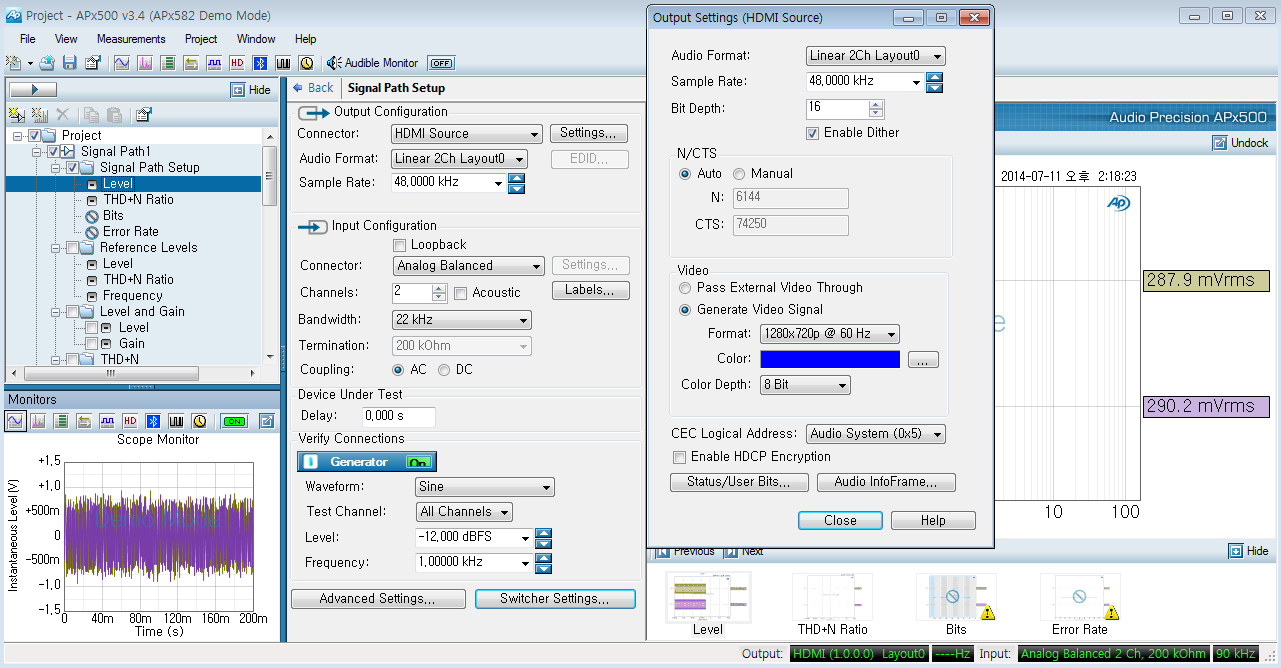
\includegraphics[width=0.9\textwidth]{figure/apsetting/signalPath.png}
\end{figure}

\end{frame}


%%%%%%%%%%%%%%%%%%%%%%%%%%%%%%%%%%%%%%%%%%%%%%%%%%%%%%%%%%%%%%%%%%%%%%%%
\begin{frame}[t]{Frequency Response Check}
\begin{itemize}
\item 테스트 신호는 Audio Precision에서 재생하는 사운드로 HDMI 혹은 unbalaced (RCA)를 이용합니다.
\item Project -> Frequency Response -> Level을 활성화 합니다.
	\begin{itemize}
	\item Start Frequency: 20Hz, Stop Frequency: 20kHz
	\item Level: -12dBFS (25\%FS, 500mVrms)
	\item Pre-Sweep: 100ms, Sweep: 3s
	\end{itemize}
\item 기능이 off일 때를 기준 (ref)으로 하고, on일 때의 출력레벨 차이값을 측정합니다.
\end{itemize}

\begin{figure}[b]
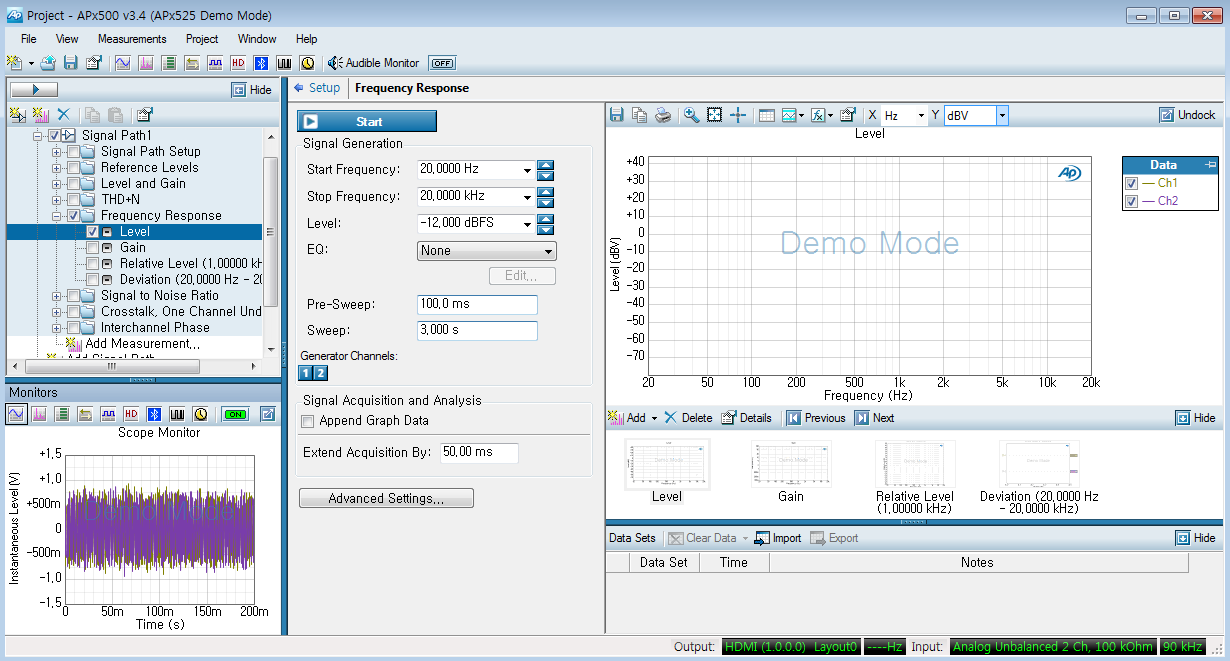
\includegraphics[width=0.9\textwidth]{figure/apsetting/frequencyResponse.png}
\end{figure}

\end{frame}


%%%%%%%%%%%%%%%%%%%%%%%%%%%%%%%%%%%%%%%%%%%%%%%%%%%%%%%%%%%%%%%%%%%%%%%%
\begin{frame}[t]{Level Check}
\begin{itemize}
\item 테스트 신호는 Audio Precision에서 재생하는 사운드로 HDMI 혹은 unbalaced (RCA)를 이용합니다.
\item Project -> Signal Path Setup -> Level을 활성화 합니다.
	\begin{itemize}
	\item Waveform: sine, Level: -12dBFS (25\%FS, 500mVrms)
	\item 스펙항목의 Frequency를 입력 합니다.
	\end{itemize}
\item 기능이 off일 때를 기준 (ref)으로 하고, on일 때 수렴한 출력레벨의 차이값을 측정합니다.
\end{itemize}

\begin{figure}[b]
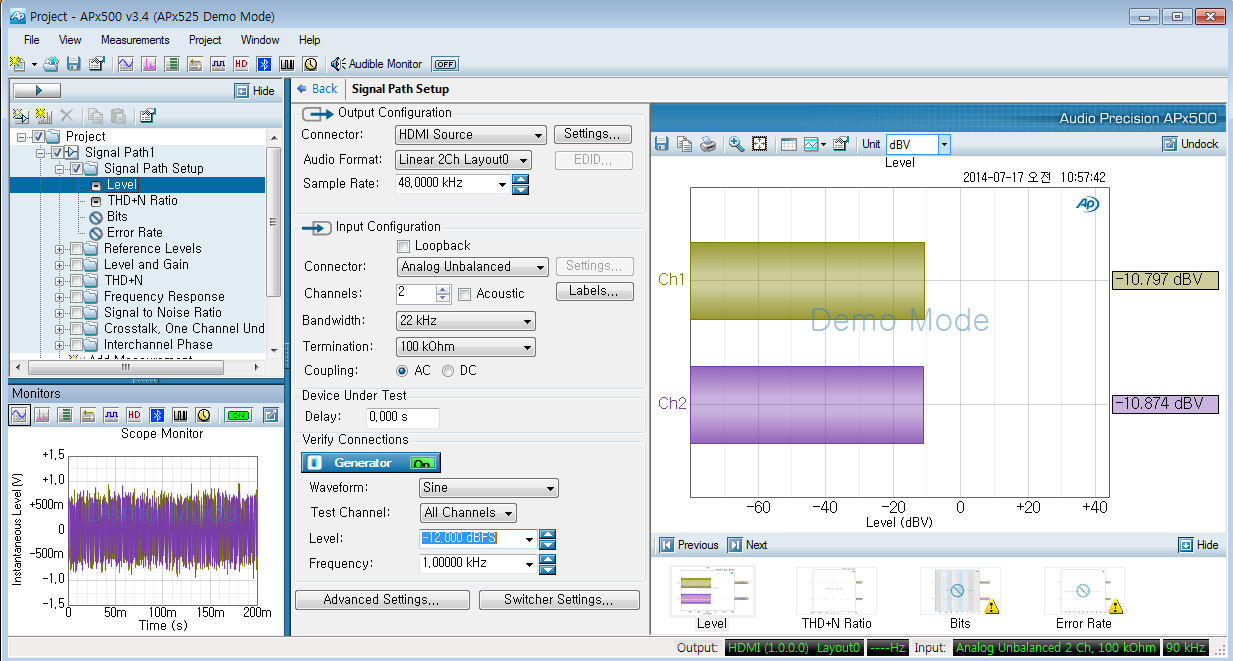
\includegraphics[width=0.9\textwidth]{figure/apsetting/level.png}
\end{figure}

\end{frame}


%%%%%%%%%%%%%%%%%%%%%%%%%%%%%%%%%%%%%%%%%%%%%%%%%%%%%%%%%%%%%%%%%%%%%%%%
\begin{frame}[t]{Fullscale Level Check}
\begin{itemize}
\item 테스트 신호는 Audio Precision에서 재생하는 사운드로 HDMI 혹은 unbalaced (RCA)를 이용합니다.
\item Project -> Signal Path Setup -> Level을 활성화 합니다.
	\begin{itemize}
	\item Waveform: sine, Level: 0dBFS (100\%FS, 2Vrms)
	\item 스펙항목의 Frequency를 입력 합니다.
	\end{itemize}
\item 기능이 off일 때를 기준 (ref)으로 하고, on일 때 수렴한 출력레벨의 차이값을 측정합니다.
\end{itemize}

\begin{figure}[b]
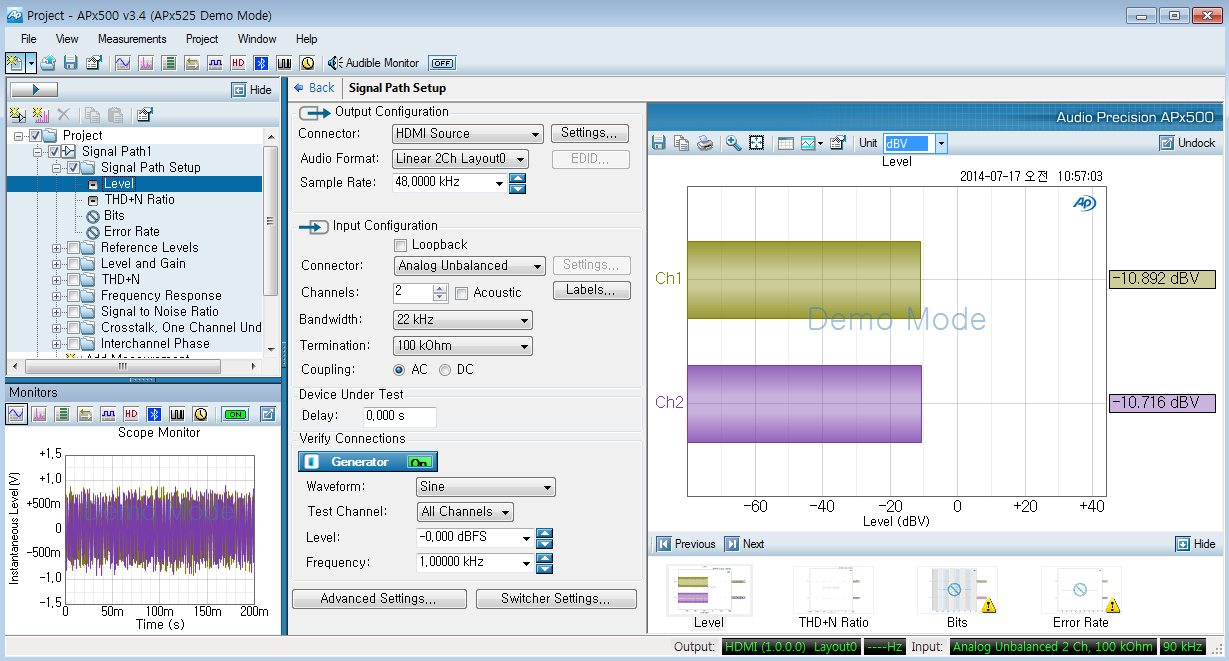
\includegraphics[width=0.9\textwidth]{figure/apsetting/fullscaleLevel.png}
\end{figure}

\end{frame}


%%%%%%%%%%%%%%%%%%%%%%%%%%%%%%%%%%%%%%%%%%%%%%%%%%%%%%%%%%%%%%%%%%%%%%%%
\begin{frame}[t]{Antiphase Level Check}
\begin{itemize}
\item 테스트 신호는 Audio Precision에서 재생하는 사운드로 HDMI 혹은 unbalaced (RCA)를 이용합니다.
\item Project -> Signal Path Setup -> Level을 활성화 합니다.
	\begin{itemize}
	\item Waveform: split phase, Level: -12dBFS (25\%FS, 500mVrms), Phase B: 180 deg
	\item 스펙항목의 Frequency를 입력 합니다.
	\end{itemize}
\item 기능이 off일 때를 기준 (ref)으로 하고, on일 때의 출력레벨 차이값을 측정합니다.
\end{itemize}

\begin{figure}[b]
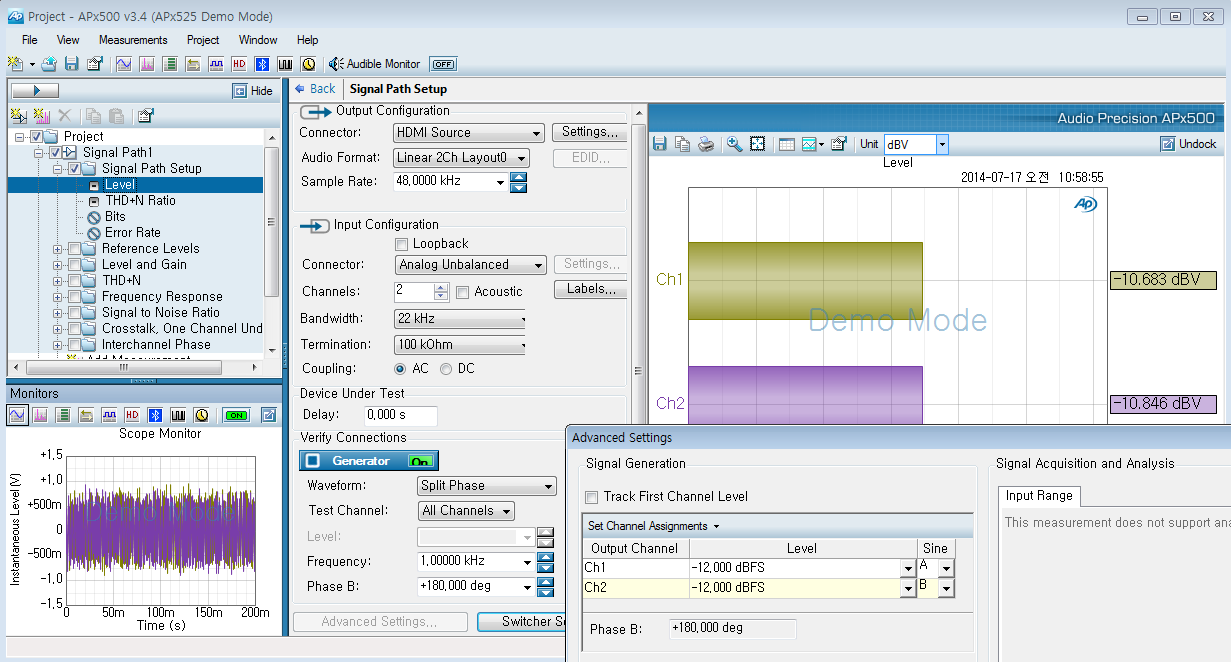
\includegraphics[width=0.9\textwidth]{figure/apsetting/antiphaseLevel.png}
\end{figure}

\end{frame}


%%%%%%%%%%%%%%%%%%%%%%%%%%%%%%%%%%%%%%%%%%%%%%%%%%%%%%%%%%%%%%%%%%%%%%%%
\begin{frame}[t]{Impulse Response Check}
\begin{itemize}
\item 테스트 신호는 Audio Precision에서 재생하는 사운드로 HDMI 혹은 unbalaced (RCA)를 이용합니다.
\item Project -> Continuous Sweep -> Impulse Response를 활성화 합니다.
  \begin{itemize}
  \item Start Frequency: 20Hz, Stop Frequency: 20kHz
  \item Level: -12dBFS (25\%FS, 500mVrms)
  \item Pre-Sweep: 100ms, Sweep: 3s
  \end{itemize}
\end{itemize}

\begin{figure}[r]
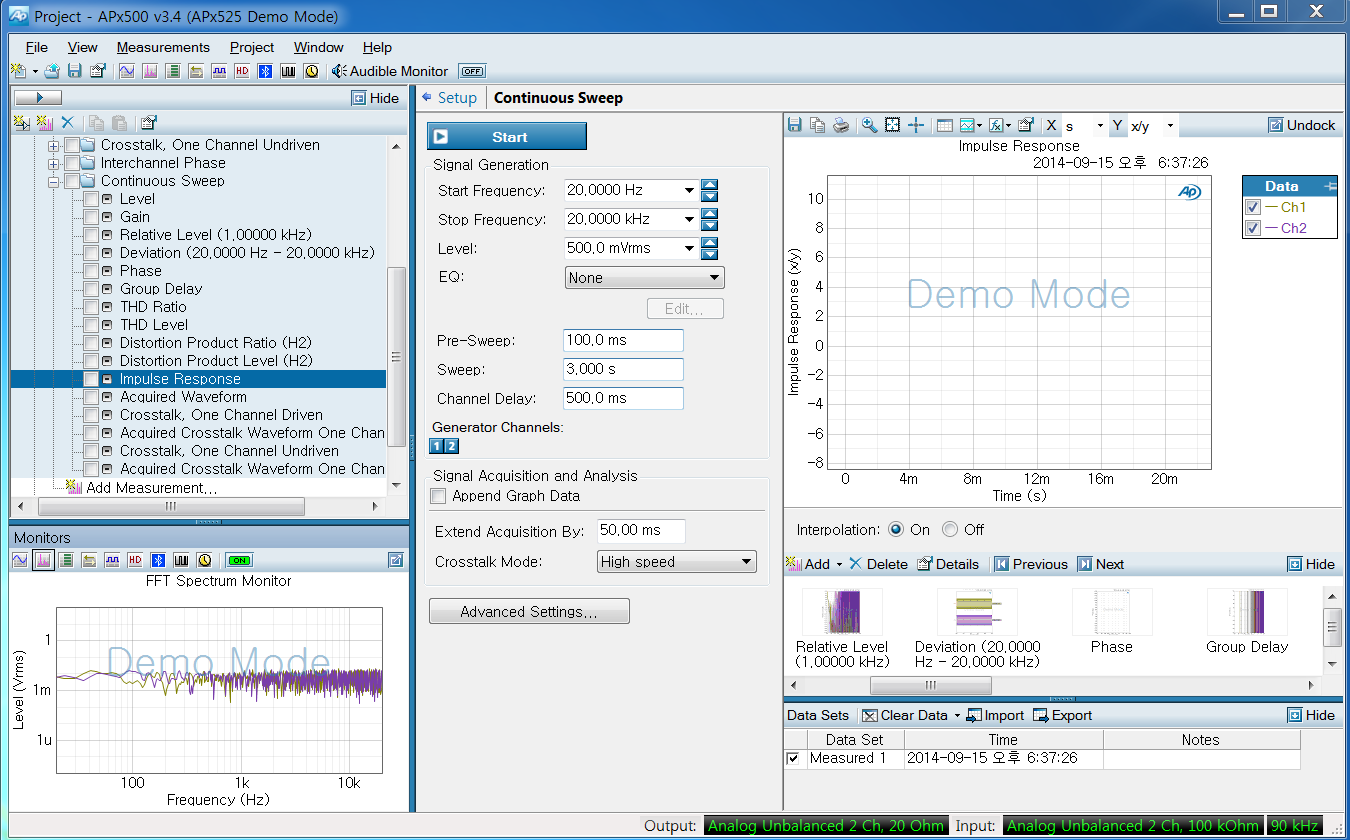
\includegraphics[width=0.9\textwidth]{figure/apsetting/impulseResponse.png}
\end{figure}

\end{frame}



%%%%%%%%%%%%%%%%%%%%%%%%%%%%%%%%%%%%%%%%%%%%%%%%%%%%%%%%%%%%%%%%%%%%%%%%
\begin{frame}[t]{Listening Test}
\begin{itemize}
\item 테스트 신호는 AP장비에서 생성하거나, 제공된 wav 혹은 mp3파일을 이용합니다.
	\begin{itemize}
	\item pink.wav
		\begin{itemize}
		\item pink noise, -20dBFS (10\%FS, 200mVrms)
		\end{itemize}
	\item pink\_antiphase.wav
		\begin{itemize}
		\item pink noise, L/R (phase: 180 deg), -20dBFS (10\%FS, 200mVrms)
		\end{itemize}
	\item sine\_fs.wav
		\begin{itemize}
		\item sine, 1kHz, 0dBFS (100\%FS, 2Vrms)
		\end{itemize}
	\end{itemize}
\item 음량의 변화나 음색의 변화를 확인합니다.
	\begin{itemize}
	\item Off 대비 음량의 변화를 확인합니다.
	\item Off 대비 상대적으로 저역대나 고역대의 레벨 변화로 인하여 음색이 변하는 것을 확인합니다.
	\end{itemize}
\end{itemize}

\end{frame}


%%%%%%%%%%%%%%%%%%%%%%%%%%%%%%%%%%%%%%%%%%%%%%%%%%%%%%%%%%%%%%%%%%%%%%%%
\begin{frame}[t]{참고}
	\begin{itemize}
	\item 본 매뉴얼은 APx500 v3.4버전 프로그램을 기준으로 작성되었습니다.
	\end{itemize}

	\begin{figure}
		\begin{center}
		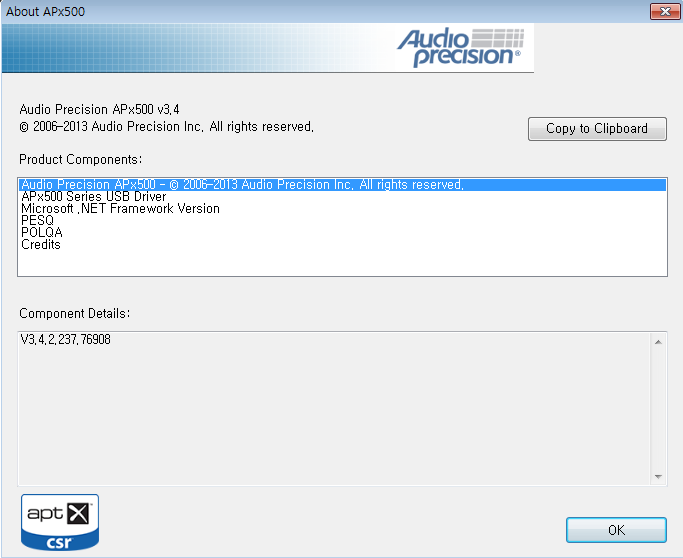
\includegraphics[width=0.7\textwidth]{figure/apsetting/apx_version.png}
		\end{center}
	\end{figure}
\end{frame}


\setbeamertemplate{itemize/enumerate body begin}{\tiny}
\setbeamertemplate{itemize/enumerate subbody begin}{\tiny}
\setbeamertemplate{itemize/enumerate subsubbody begin}{\tiny}

%%%%%%%%%%%%%%%%%%%%%%%%%%%%%%%%%%%%%%%%%%%%%%%%%%%%%%%%%%%%%%%%%%%%%%%%
\begin{frame}[t]{Clearvoice: level +1}
\begin{tiny}
\begin{tabular}{@{}lccc@{}}
\toprule
Function & Off/On & Option & Specification \\
\midrule
Audio AMP EQ & \color{black}{Off} & Instart &
\multirow{13}{60mm}{
\begin{itemize}
\item Remark
	\begin{itemize}
	\item 목소리를 명료하게 하는 기능
	\item L/R 채널의 primary (목소리)와 ambient 성분(배경음, 잔향)을 분리하여 EQ 적용
	\end{itemize}
\item Listening Test (pink.wav)
	\begin{itemize}
	\item 음색의 변화: Off 대비 저역대의 레벨 증가
	\end{itemize}
\item Frequency Response Check
  \begin{itemize}
  \item 20Hz-500Hz에서 ref 신호와의 레벨 차이값이 +10±1dBr 이내
  \item 800Hz-20kHz에서 ref 신호와의 레벨 차이값이 0±1dBr 이내
  \end{itemize}
\end{itemize}
} \\
Clearvoice & \color{blue}{On} & \color{blue}{+1} & \\
Autovolume & \color{black}{Off} & & \\
Sound Mode & \color{black}{Off} & & \\
Sound Optimizer & \color{black}{Off} & & \\
Height Channel & \color{black}{Off} & & \\
Automatic Scene Classificiation & \color{black}{Off} & & \\
Limiter & \color{black}{Off} & & \\
Sound Stage Expansion & \color{black}{Off} & & \\
Dynamic Range Control & \color{black}{Off} & & \\
Smart Sound Controller & \color{black}{Off} & & \\
High Resolution & \color{black}{Off} & & \\
OSD Volume & \color{blue}{On} & Vol.40 & \\
\midrule
\end{tabular}
\end{tiny}

\begin{figure}[b]
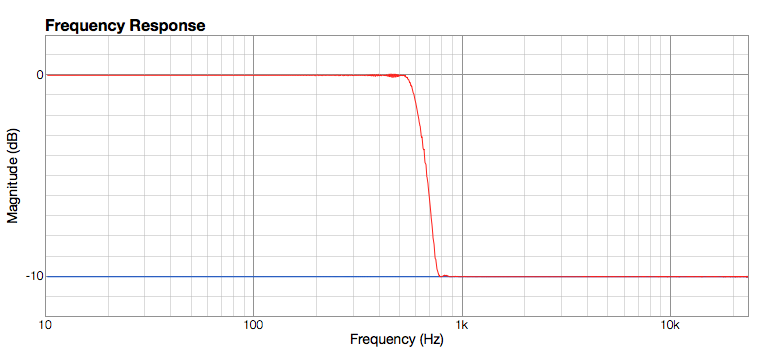
\includegraphics[height=0.37\textwidth]{figure/cv1.png}
\end{figure}

\end{frame}


%%%%%%%%%%%%%%%%%%%%%%%%%%%%%%%%%%%%%%%%%%%%%%%%%%%%%%%%%%%%%%%%%%%%%%%%
\begin{frame}[t]{Clearvoice: level +2}
\begin{tiny}
\begin{tabular}{@{}lccc@{}}
\toprule
Function & Off/On & Option & Specification \\
\midrule
Audio AMP EQ & \color{black}{Off} & Instart &
\multirow{13}{60mm}{
\begin{itemize}
\item Remark
	\begin{itemize}
	\item 목소리를 명료하게 하는 기능
	\item L/R 채널의 primary (목소리)와 ambient 성분(배경음, 잔향)을 분리하여 EQ 적용
	\end{itemize}
\item Listening Test (pink.wav)
	\begin{itemize}
	\item Off 대비 저역대의 음량 증가
	\item 음색의 변화: level1보다 고역대의 레벨 증가
	\end{itemize}
\item Frequency Response Check
  \begin{itemize}
  \item 20Hz-1.5kHz에서 ref 신호와의 레벨 차이값이 +10±1dBr 이내
  \item 2kHz-20kHz에서 ref 신호와의 레벨 차이값이 0±1dBr 이내
  \end{itemize}
\end{itemize}
} \\
Clearvoice & \color{blue}{On} & \color{blue}{+2} & \\
Autovolume & \color{black}{Off} & & \\
Sound Mode & \color{black}{Off} & & \\
Sound Optimizer & \color{black}{Off} & & \\
Height Channel & \color{black}{Off} & & \\
Automatic Scene Classificiation & \color{black}{Off} & & \\
Limiter & \color{black}{Off} & & \\
Sound Stage Expansion & \color{black}{Off} & & \\
Dynamic Range Control & \color{black}{Off} & & \\
Smart Sound Controller & \color{black}{Off} & & \\
High Resolution & \color{black}{Off} & & \\
OSD Volume & \color{blue}{On} & Vol.40 & \\
\midrule
\end{tabular}
\end{tiny}

\begin{figure}[b]
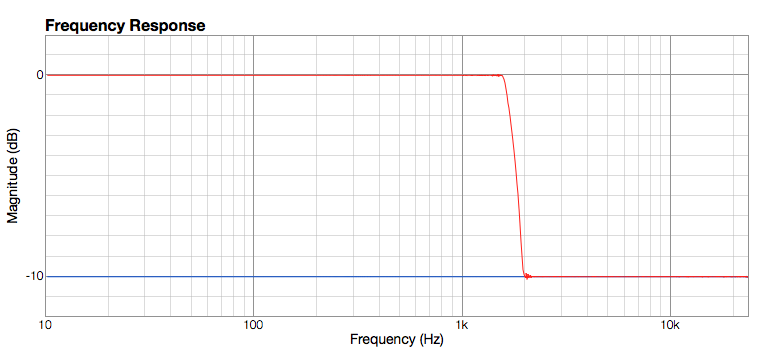
\includegraphics[height=0.37\textwidth]{figure/cv2.png}
\end{figure}

\end{frame}


%%%%%%%%%%%%%%%%%%%%%%%%%%%%%%%%%%%%%%%%%%%%%%%%%%%%%%%%%%%%%%%%%%%%%%%%
\begin{frame}[t]{Clearvoice: level +3}
\begin{tiny}
\begin{tabular}{@{}lccc@{}}
\toprule
Function & Off/On & Option & Specification \\
\midrule
Audio AMP EQ & \color{black}{Off} & Instart &
\multirow{13}{60mm}{
\begin{itemize}
\item Remark
	\begin{itemize}
	\item 목소리를 명료하게 하는 기능
	\item L/R 채널의 primary (목소리)와 ambient 성분(배경음, 잔향)을 분리하여 EQ 적용
	\end{itemize}
\item Listening Test (pink.wav)
	\begin{itemize}
	\item Off 대비 음량 증가
	\item 음색의 변화: level2보다 고역대의 레벨 증가
	\end{itemize}
\item Frequency Response Check
  \begin{itemize}
  \item 20Hz-9kHz에서 ref 신호와의 레벨 차이값이 +10±1dBr 이내
  \item 12kHz-20kHz에서 ref 신호와의 레벨 차이값이 0±1dBr 이내
  \end{itemize}
\end{itemize}
} \\
Clearvoice & \color{blue}{On} & \color{blue}{+3} & \\
Autovolume & \color{black}{Off} & & \\
Sound Mode & \color{black}{Off} & & \\
Sound Optimizer & \color{black}{Off} & & \\
Height Channel & \color{black}{Off} & & \\
Automatic Scene Classificiation & \color{black}{Off} & & \\
Limiter & \color{black}{Off} & & \\
Sound Stage Expansion & \color{black}{Off} & & \\
Dynamic Range Control & \color{black}{Off} & & \\
Smart Sound Controller & \color{black}{Off} & & \\
High Resolution & \color{black}{Off} & & \\
OSD Volume & \color{blue}{On} & Vol.40 & \\
\midrule
\end{tabular}
\end{tiny}

\begin{figure}[b]
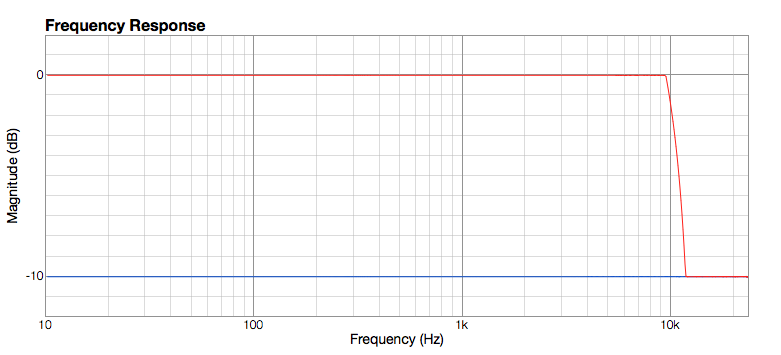
\includegraphics[height=0.37\textwidth]{figure/cv3.png}
\end{figure}

\end{frame}


%%%%%%%%%%%%%%%%%%%%%%%%%%%%%%%%%%%%%%%%%%%%%%%%%%%%%%%%%%%%%%%%%%%%%%%%
\begin{frame}[t]{Autovolume}
\begin{tiny}
\begin{tabular}{@{}lccc@{}}
\toprule
Function & Off/On & Option & Specification \\
\midrule
Audio AMP EQ & \color{black}{Off} & Instart &
\multirow{13}{60mm}{
\begin{itemize}
\item Remark
	\begin{itemize}
	\item 음량을 정규화 하는 기능
	\item 볼륨이 큰 소리는 작게, 작은 소리는 크게 조절
	\end{itemize}
\item Listening Test (pink.wav)
	\begin{itemize}
	\item Off 대비 전대역의 음량 감소
	\item 음색의 변화 없음
	\end{itemize}
\item Level Check
  \begin{itemize}
  \item 1kHz에서 ref 신호와의 레벨 차이값이 -12±2dBr 이내
  \item 10kHz에서 ref 신호와의 레벨 차이값이 -12±2dBr 이내
  \end{itemize}
\end{itemize}
} \\
Clearvoice & \color{black}{Off} & & \\
Autovolume & \color{blue}{On} & & \\
Sound Mode & \color{black}{Off} & & \\
Sound Optimizer & \color{black}{Off} & & \\
Height Channel & \color{black}{Off} & & \\
Automatic Scene Classificiation & \color{black}{Off} & & \\
Limiter & \color{black}{Off} & & \\
Sound Stage Expansion & \color{black}{Off} & & \\
Dynamic Range Control & \color{black}{Off} & & \\
Smart Sound Controller & \color{black}{Off} & & \\
High Resolution & \color{black}{Off} & & \\
OSD Volume & \color{blue}{On} & Vol.40 & \\
\midrule
\end{tabular}
\end{tiny}

\end{frame}


%%%%%%%%%%%%%%%%%%%%%%%%%%%%%%%%%%%%%%%%%%%%%%%%%%%%%%%%%%%%%%%%%%%%%%%%
\begin{frame}[t]{Sound Mode}
\begin{tiny}
\begin{tabular}{@{}lccc@{}}
\toprule
Function & Off/On & Option & Specification \\
\midrule
Audio AMP EQ & \color{black}{Off} & Instart &
\multirow{13}{60mm}{
\begin{itemize}
\item Remark
	\begin{itemize}
	\item 5-band PEQ를 이용하여 다양한 음향효과를 적용하는 기능
	\item 다양한 음향 모드 (뉴스, 음악, 영화, 스포츠, 게임)를 지원
	\end{itemize}
\item Listening Test (pink.wav)
	\begin{itemize}
	\item Off 대비 음량 감소
	\item 음색의 변화
	\end{itemize}
\item Frequency Response Check
  \begin{itemize}
  \item convex 형태 (U형)의 주파수응답
  \item 1kHz에서 ref 신호와의 레벨 차이값이 -10±1dBr 이내
  \end{itemize}
\end{itemize}
} \\
Clearvoice & \color{black}{Off} & & \\
Autovolume & \color{black}{Off} & & \\
Sound Mode & \color{blue}{On} & & \\
Sound Optimizer & \color{black}{Off} & & \\
Height Channel & \color{black}{Off} & & \\
Automatic Scene Classificiation & \color{black}{Off} & & \\
Limiter & \color{black}{Off} & & \\
Sound Stage Expansion & \color{black}{Off} & & \\
Dynamic Range Control & \color{black}{Off} & & \\
Smart Sound Controller & \color{black}{Off} & & \\
High Resolution & \color{black}{Off} & & \\
OSD Volume & \color{blue}{On} & Vol.40 & \\
\midrule
\end{tabular}
\end{tiny}

\begin{figure}[b]
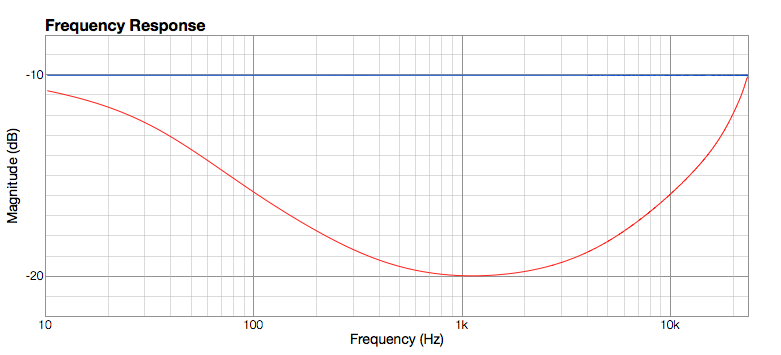
\includegraphics[height=0.37\textwidth]{figure/soundmode.png}
\end{figure}

\end{frame}


%%%%%%%%%%%%%%%%%%%%%%%%%%%%%%%%%%%%%%%%%%%%%%%%%%%%%%%%%%%%%%%%%%%%%%%%
\begin{frame}[t]{Sound Optimizer}
\begin{tiny}
\begin{tabular}{@{}lccc@{}}
\toprule
Function & Off/On & Option & Specification \\
\midrule
Audio AMP EQ & \color{black}{Off} & Instart &
\multirow{13}{60mm}{
\begin{itemize}
\item Remark
	\begin{itemize}
	\item 3-band PEQ를 이용하여 TV의 설치 방식 (벽걸이, 스탠드)에 따른 음질변화를 보상하는 기능
	\end{itemize}
\item Listening Test (pink.wav)
	\begin{itemize}
	\item off 대비 음량 변화의 인지가 어려움
	\item 음색의 변화: 저역대와 고역대의 레벨 감소
	\end{itemize}
\item Frequency Response Check
  \begin{itemize}
  \item concave 형태 (n형)의 주파수응답
  \item 1kHz에서 ref 신호와의 레벨 차이값이 6±1dBr 이내
  \end{itemize}
\end{itemize}
} \\
Clearvoice & \color{black}{Off} & & \\
Autovolume & \color{black}{Off} & & \\
Sound Mode & \color{black}{Off} & & \\
Sound Optimizer & \color{blue}{On} & & \\
Height Channel & \color{black}{Off} & & \\
Automatic Scene Classificiation & \color{black}{Off} & & \\
Limiter & \color{black}{Off} & & \\
Sound Stage Expansion & \color{black}{Off} & & \\
Dynamic Range Control & \color{black}{Off} & & \\
Smart Sound Controller & \color{black}{Off} & & \\
High Resolution & \color{black}{Off} & & \\
OSD Volume & \color{blue}{On} & Vol.40 & \\
\midrule
\end{tabular}
\end{tiny}

\begin{figure}[b]
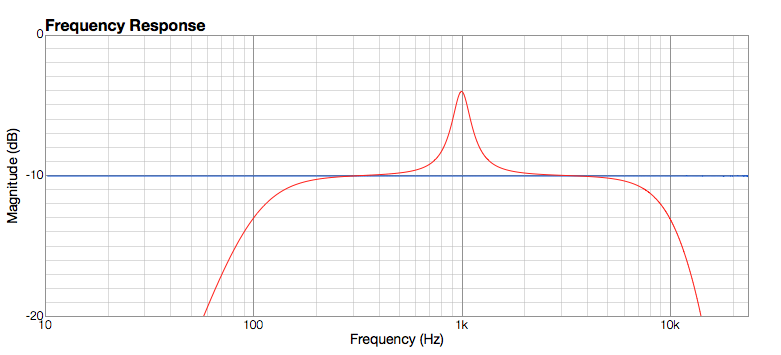
\includegraphics[height=0.37\textwidth]{figure/soundoptimizer.png}
\end{figure}

\end{frame}


%%%%%%%%%%%%%%%%%%%%%%%%%%%%%%%%%%%%%%%%%%%%%%%%%%%%%%%%%%%%%%%%%%%%%%%%
\begin{frame}[t]{Height Channel}
\begin{tiny}
\begin{tabular}{@{}lccc@{}}
\toprule
Function & Off/On & Option & Specification \\
\midrule
Audio AMP EQ & \color{black}{Off} & Instart &
\multirow{13}{60mm}{
\begin{itemize}
\item Remark
	\begin{itemize}
	\item 3차원 음향효과 (공간감, 잔향감)를 제공하는 기능
	\item 반사, 잔향음을 조절
	\end{itemize}
\item Listening Test (pink\_antiphase.wav)
	\begin{itemize}
	\item Off 대비 음량 증가
	\item 음색의 변화: 고역대 레벨 증가
	\end{itemize}
\item Antiphase Level Check
  \begin{itemize}
  \item 1kHz에서 ref 신호와의 레벨 차이값이 9.5±3dBr 이내
  \item 5kHz에서 ref 신호와의 레벨 차이값이 11.3±3dBr 이내
  \item 10kHz에서 ref 신호와의 레벨 차이값이 12±3dBr 이내
  \end{itemize}
\end{itemize}
} \\
Clearvoice & \color{black}{Off} & & \\
Autovolume & \color{black}{Off} & & \\
Sound Mode & \color{black}{Off} & & \\
Sound Optimizer & \color{black}{Off} & & \\
Height Channel & \color{blue}{On} & & \\
Automatic Scene Classificiation & \color{black}{Off} & & \\
Limiter & \color{black}{Off} & & \\
Sound Stage Expansion & \color{black}{Off} & & \\
Dynamic Range Control & \color{black}{Off} & & \\
Smart Sound Controller & \color{black}{Off} & & \\
High Resolution & \color{black}{Off} & & \\
OSD Volume & \color{blue}{On} & Vol.40 & \\
\midrule
\end{tabular}
\end{tiny}

\end{frame}


%%%%%%%%%%%%%%%%%%%%%%%%%%%%%%%%%%%%%%%%%%%%%%%%%%%%%%%%%%%%%%%%%%%%%%%%
\begin{frame}[t]{Sound Stage Expansion}
\begin{tiny}
\begin{tabular}{@{}lccc@{}}
\toprule
Function & Off/On & Option & Specification \\
\midrule
Audio AMP EQ & \color{black}{Off} & Instart &
\multirow{13}{60mm}{
\begin{itemize}
\item Remark
	\begin{itemize}
	\item 3차원 음향효과 (공간감, 현장감)를 제공하는 기능
	\item 입력 2채널을 이용하여 최대 8채널 업믹스하는 기능
	\item L/R 채널의 primary 성분 (목소리)과 ambient 성분(배경음, 잔향)을 조절
	\end{itemize}
\item Listening Test (pink.wav)
	\begin{itemize}
	\item Off 대비 음량 감소
	\item 음색의 변화: 저역대의 레벨 감소
	\end{itemize}
\item Frequency Response Check
  \begin{itemize}
  \item 20Hz-1.5kHz에서 ref 신호와의 레벨 차이값이 -10±1dBr 이내
  \item 3kHz-20kHz에서 ref 신호와의 레벨 차이값이 0±1dBr 이내
  \end{itemize}
\end{itemize}
} \\
Clearvoice & \color{black}{Off} & & \\
Autovolume & \color{black}{Off} & & \\
Sound Mode & \color{black}{Off} & & \\
Sound Optimizer & \color{black}{Off} & & \\
Height Channel & \color{black}{Off} & & \\
Automatic Scene Classificiation & \color{black}{Off} & & \\
Limiter & \color{black}{Off} & & \\
Sound Stage Expansion & \color{blue}{On} & & \\
Dynamic Range Control & \color{black}{Off} & & \\
Smart Sound Controller & \color{black}{Off} & & \\
High Resolution & \color{black}{Off} & & \\
OSD Volume & \color{blue}{On} & Vol.40 & \\
\midrule
\end{tabular}
\end{tiny}

\begin{figure}[b]
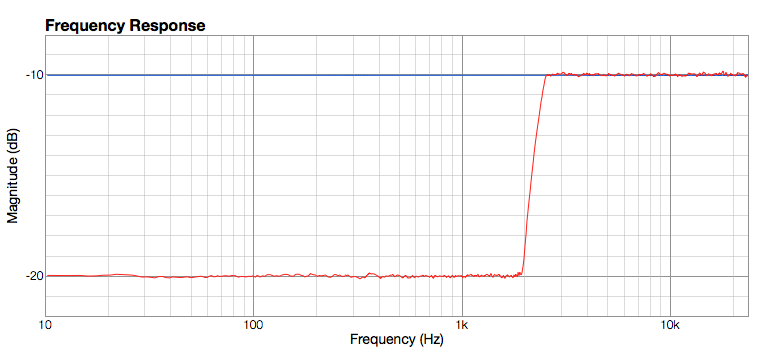
\includegraphics[height=0.37\textwidth]{figure/sxp.png}
\end{figure}

\end{frame}


%%%%%%%%%%%%%%%%%%%%%%%%%%%%%%%%%%%%%%%%%%%%%%%%%%%%%%%%%%%%%%%%%%%%%%%%
\begin{frame}[t]{Smart Sound}
\begin{tiny}
\begin{tabular}{@{}lccc@{}}
\toprule
Function & Off/On & Option & Specification \\
\midrule
Audio AMP EQ & \color{black}{Off} & Instart &
\multirow{13}{60mm}{
\begin{itemize}
\item Remark
	\begin{itemize}
	\item 음원의 장르적 패턴 (목소리/음악/효과음의 확률)을 분석하여 음향효과를 적용하는 자동음장 기능
	\end{itemize}
\item Listening Test (pink.wav)
	\begin{itemize}
	\item Off 대비 음량 증가
	\item 음량이 서서히 변화
	\item 음색의 변화 없음
	\end{itemize}
\item Level Check
  \begin{itemize}
  \item 50Hz에서 ref 신호와의 레벨 차이값이 1.5±2dBr 이내
  \item 100Hz에서 ref 신호와의 레벨 차이값이 4.5±2dBr 이내
  \end{itemize}
\end{itemize}
} \\
Clearvoice & \color{black}{Off} & & \\
Autovolume & \color{black}{Off} & & \\
Sound Mode & \color{black}{Off} & & \\
Sound Optimizer & \color{black}{Off} & & \\
Height Channel & \color{black}{Off} & & \\
Automatic Scene Classificiation & \color{blue}{On} & & \\
Limiter & \color{black}{Off} & & \\
Sound Stage Expansion & \color{blue}{On} & & \\
Dynamic Range Control & \color{black}{Off} & & \\
Smart Sound Controller & \color{blue}{On} & & \\
High Resolution & \color{black}{Off} & & \\
OSD Volume & \color{blue}{On} & Vol.40 & \\
\midrule
\end{tabular}
\end{tiny}

\end{frame}


%%%%%%%%%%%%%%%%%%%%%%%%%%%%%%%%%%%%%%%%%%%%%%%%%%%%%%%%%%%%%%%%%%%%%%%%
\begin{frame}[t]{Limiter}
\begin{tiny}
\begin{tabular}{@{}lccc@{}}
\toprule
Function & Off/On & Option & Specification \\
\midrule
Audio AMP EQ & \color{black}{Off} & Instart &
\multirow{13}{60mm}{
\begin{itemize}
\item Remark
	\begin{itemize}
	\item 클리핑을 방지하며 헤드룸의 음량 손실을 보상하는 기능
	\end{itemize}
\item Listening Test (sin\_fs.wav)
	\begin{itemize}
	\item Off 대비 음량 감소
	\item 음량이 천천히 수렴
	\end{itemize}
\item Level Check
  \begin{itemize}
  \item 1kHz에서 ref 신호와의 레벨 차이값이 -6dBr 이하
  \item 10kHz에서 ref 신호와의 레벨 차이값이 -6dBr 이하
  \end{itemize}
\end{itemize}
} \\
Clearvoice & \color{black}{Off} & & \\
Autovolume & \color{black}{Off} & & \\
Sound Mode & \color{black}{Off} & & \\
Sound Optimizer & \color{black}{Off} & & \\
Height Channel & \color{black}{Off} & & \\
Automatic Scene Classificiation & \color{black}{Off} & & \\
Limiter & \color{blue}{On} & & \\
Sound Stage Expansion & \color{black}{Off} & & \\
Dynamic Range Control & \color{black}{Off} & & \\
Smart Sound Controller & \color{black}{Off} & & \\
High Resolution & \color{black}{Off} & & \\
OSD Volume & \color{blue}{On} & Vol.40 & \\
\midrule
\end{tabular}
\end{tiny}

\end{frame}


%%%%%%%%%%%%%%%%%%%%%%%%%%%%%%%%%%%%%%%%%%%%%%%%%%%%%%%%%%%%%%%%%%%%%%%%
\begin{frame}[t]{Dynamic Range Control}
\begin{tiny}
\begin{tabular}{@{}lccc@{}}
\toprule
Function & Off/On & Option & Specification \\
\midrule
Audio AMP EQ & \color{black}{Off} & Instart &
\multirow{13}{60mm}{
\begin{itemize}
\item Remark
	\begin{itemize}
	\item 신호의 Dynamic Range와 음량을 대역별로 제어하는 기능
	\end{itemize}
\item Listening Test (sine\_fs.wav)
	\begin{itemize}
	\item Off 대비 음량 변화의 인지가 어려움
	\item 음색의 변화: 중역대의 레벨 증가
	\end{itemize}
\item Frequency Response Check
  \begin{itemize}
  \item 20-600Hz에서 ref 신호와의 레벨 차이값이 0±1dBr 이내
  \item 1kHz-6kHz에서 ref 신호와의 레벨 차이값이 6dBr 이상
  \item 8kHz-20kHz에서 ref 신호와의 레벨 차이값이 -6dBr 이하
  \end{itemize}
\end{itemize}
} \\
Clearvoice & \color{black}{Off} & & \\
Autovolume & \color{black}{Off} & & \\
Sound Mode & \color{black}{Off} & & \\
Sound Optimizer & \color{black}{Off} & & \\
Height Channel & \color{black}{Off} & & \\
Automatic Scene Classificiation & \color{black}{Off} & & \\
Limiter & \color{black}{Off} & & \\
Sound Stage Expansion & \color{black}{Off} & & \\
Dynamic Range Control & \color{blue}{On} & & \\
Smart Sound Controller & \color{black}{Off} & & \\
High Resolution & \color{black}{Off} & & \\
OSD Volume & \color{blue}{On} & Vol.40 & \\
\midrule
\end{tabular}
\end{tiny}

\begin{figure}[b]
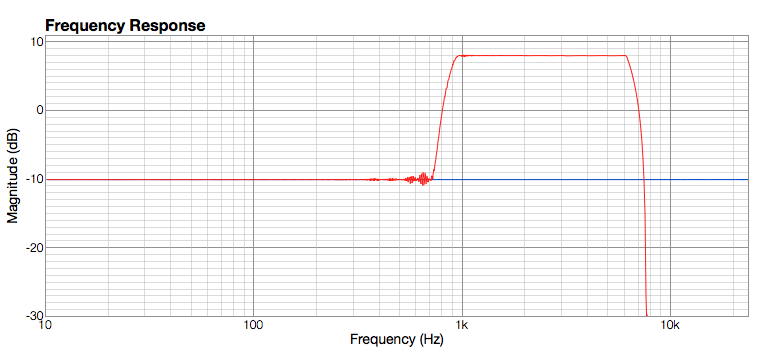
\includegraphics[height=0.37\textwidth]{figure/drc.png}
\end{figure}

\end{frame}


%%%%%%%%%%%%%%%%%%%%%%%%%%%%%%%%%%%%%%%%%%%%%%%%%%%%%%%%%%%%%%%%%%%%%%%%
\begin{frame}[t]{High Resolution}
\begin{tiny}
\begin{tabular}{@{}lccc@{}}
\toprule
Function & Off/On & Option & Specification \\
\midrule
Audio AMP EQ & \color{black}{Off} & Instart &
\multirow{13}{60mm}{
\begin{itemize}
\item Remark
  \begin{itemize}
  \item 고해상도 기능 (96kHz를 지원, 스피커의 대역별 Phase 특성을 보상, 공간적 특성을 반영)
  \end{itemize}
\item Listening Test (voice.wav)
  \begin{itemize}
  \item Off 대비 음량 변화의 인지가 어려움
  \item Off 대비 에코처럼 울림현상
  \end{itemize}
\end{itemize}
} \\
Clearvoice & \color{black}{Off} & & \\
Autovolume & \color{black}{Off} & & \\
Sound Mode & \color{black}{Off} & & \\
Sound Optimizer & \color{black}{Off} & & \\
Height Channel & \color{black}{Off} & & \\
Automatic Scene Classificiation & \color{black}{Off} & & \\
Limiter & \color{black}{Off} & & \\
Sound Stage Expansion & \color{black}{Off} & & \\
Dynamic Range Control & \color{black}{Off} & & \\
Smart Sound Controller & \color{black}{Off} & & \\
High Resolution & \color{blue}{On} & & \\
OSD Volume & \color{blue}{On} & Vol.40 & \\
\midrule
\end{tabular}
\end{tiny}

\end{frame}

%%%%%%%%%%%%%%%%%%%%%%%%%%%%%%%%%%%%%%%%%%%%%%%%%%%%%%%%%%%%%%%%%%%%%%%%
\begin{frame}[t]{High Resolution}
\begin{tiny}
\begin{tabular}{@{}lccc@{}}
\toprule
Function & Off/On & Option & Specification \\
\midrule
Audio AMP EQ & \color{black}{Off} & Instart &
\multirow{13}{60mm}{
\begin{itemize}
\item Impulse Response Check
  \begin{itemize}
  \item max impulse를 ref로 정의 (시간: 0s, 크기: 1.0)
  \item 8.5±1ms구간의 max impulse가 ref대비 0.14±0.05 이내
  \item 11.5±1ms구간의 max impulse가 ref대비 0.14±0.05 이내
  \item 14.5±1ms구간의 max impulse가 ref대비 0.14±0.05 이내
  \item 18.5±1ms구간의 max impulse가 ref대비 0.14-0.05 이내
  \item 1-2번째의 impulse에서 impulse의 envelope이 서서히 변화
  \item 주요한 impulse는 위의 5구간에서만 나타나며, 20ms 이후의 impulse는 분석하지 않음
  \item Left/Right의 3rd, 4th impulse는 허용오차 범위내에서 측정 결과가 다름
  \item AMP와 AP의 연결방법에 의하여 y축 대칭의 결과가 발생
  \end{itemize}
\end{itemize}
} \\
Clearvoice & \color{black}{Off} & & \\
Autovolume & \color{black}{Off} & & \\
Sound Mode & \color{black}{Off} & & \\
Sound Optimizer & \color{black}{Off} & & \\
Height Channel & \color{black}{Off} & & \\
Automatic Scene Classificiation & \color{black}{Off} & & \\
Limiter & \color{black}{Off} & & \\
Sound Stage Expansion & \color{black}{Off} & & \\
Dynamic Range Control & \color{black}{Off} & & \\
Smart Sound Controller & \color{black}{Off} & & \\
High Resolution & \color{blue}{On} & & \\
OSD Volume & \color{blue}{On} & Vol.40 & \\
\midrule
\end{tabular}
\end{tiny}

\begin{figure}[b]
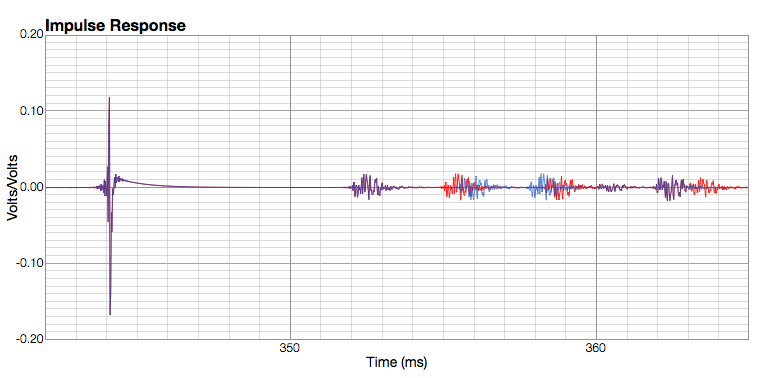
\includegraphics[height=0.37\textwidth]{figure/highresolution.png}
\end{figure}

\end{frame}



\end{document}
